\section{Rekomendasi Kebijakan: Program Pasangan Kuota PLTS Atap dan Pensiun Dini}
\label{sec:rekomendasi}

\subsection{Gambaran Program}

Untuk menjawab keenam celah pada Bab~\ref{sec:celah}, kajian ini merekomendasikan program pasangan kuota PLTS atap dan pensiun dini PLTU. Program ini menjabarkan solusi terpilih laporan kelompok menjadi aturan yang dapat dijalankan. Setiap PLTU yang dipensiunkan dipasangkan dengan tambahan PLTS atap paling sedikit setara dayanya, dan penutupan baru dilakukan setelah dana, pengganti, dan program pekerja siap.

Program ini berpegang pada lima prinsip:
\begin{enumerate}
  \item \textbf{Berpasangan}, yaitu kuota PLTS atap dihitung dari rencana pensiun dini, bukan ditetapkan terpisah.
  \item \textbf{Hemat bagi negara}, yaitu PLTU dipilih berdasarkan dampaknya terhadap neraca negara per GW, sehingga pensiun dini PLTU IPP didahulukan.
  \item \textbf{Bersyarat}, yaitu penutupan dilakukan hanya setelah dana luar terikat, pembangkit pengganti siap, dan pekerja tercakup program.
  \item \textbf{Berbagi beban}, yaitu investasi PLTS atap disebar ke APBN, BUMN, dan swasta melalui kewajiban dan insentif.
  \item \textbf{Terbuka}, yaitu setiap usulan dinilai dengan alat hitung yang sama dan dapat diperiksa ulang.
\end{enumerate}

\subsection{Komponen Program}

Program terdiri atas enam komponen. Setiap komponen menjawab satu atau lebih celah kebijakan (Tabel~\ref{tab:komponen}).

\begin{table}[H]
\centering
\caption{Komponen program pasangan kuota PLTS atap dan pensiun dini}
\label{tab:komponen}
\small
\begin{tabularx}{\textwidth}{L{0.7cm} L{3.3cm} Y L{1.9cm}}
\toprule
Kode & Komponen & Isi utama & Celah \\
\midrule
K1 & Kuota berpasangan & Kuota PLTS atap tahunan di suatu sistem paling sedikit sama dengan kapasitas PLTU yang dijadwalkan pensiun di sistem tersebut & 1 \\
\addlinespace
K2 & Kewajiban dan insentif PLTS atap & Mulai 2028, gedung pemerintah dan BUMN di Jawa-Bali wajib memasang 200 MW per tahun. Industri memperoleh insentif fiskal 15\% dari harga pemasangan & 1 \\
\addlinespace
K3 & Urutan pensiun dini & PLTU dipilih dari daftar urut neraca negara per GW. PLTU IPP berdampak kesehatan tinggi didahulukan, PLTU milik PLN ditunda ke Fase 4 & 2 \\
\addlinespace
K4 & Syarat penutupan & Dana luar paling sedikit 80\% kompensasi terikat dan pembangkit pengganti beroperasi sebelum tanggal penutupan & 3, 4 \\
\addlinespace
K5 & Transisi pekerja & Pelatihan ulang dan perlindungan sosial bagi pekerja PLTU dimulai paling lambat satu tahun sebelum penutupan, diarahkan ke pemasangan dan pemeliharaan PLTS atap & 5 \\
\addlinespace
K6 & Alat hitung bersama PowerShift & Platform terbuka untuk menyaring kandidat, menguji paket, dan memantau indikator roadmap dengan data dan rumus yang sama bagi semua pihak & 6 \\
\bottomrule
\end{tabularx}
\end{table}

\subsection{Mekanisme Pasangan dan Syarat Penutupan}

Komponen K1, K3, dan K4 membentuk mekanisme inti program. Untuk setiap PLTU yang diusulkan pensiun pada tahun $Y$, Satgas memeriksa empat syarat berikut.
\begin{enumerate}
  \item \textbf{Neraca negara per GW tidak negatif} pada penyaringan kandidat di PowerShift. Syarat ini memastikan pensiun dini tidak membebani APBN dalam horizon kajian.
  \item \textbf{Rencana tambahan PLTS atap} hingga akhir roadmap (2040) paling sedikit sama dengan seluruh kapasitas PLTU yang dipensiunkan, dengan lintasan tahunan yang dipantau. Selama PLTS atap masih tertinggal, kekurangannya ditutup pembangkit pengganti pada syarat keempat.
  \item \textbf{Dana luar terikat} paling sedikit 80\% dari kompensasi.
  \item \textbf{Pembangkit pengganti siap} sebesar kapasitas yang diperlukan agar reserve margin tetap 33\%.
\end{enumerate}

Sebagai ilustrasi, Cirebon-1 (660 MW, IPP) yang dipensiunkan pada 2030 memerlukan kompensasi sekitar Rp0,69 triliun per tahun percepatan dengan estimasi skema ETM, atau Rp7,6 triliun selama 2030-2040. Dengan 80\% dari dana luar, porsi PLN Rp1,5 triliun dan dana luar Rp6,1 triliun. Pada saat yang sama, PLN berhenti membayar kapasitas Cirebon-1. Bila dipensiunkan sendiri, Cirebon-1 memberi neraca negara positif Rp4,3 triliun, atau Rp6,5 triliun per GW, sehingga syarat pertama terpenuhi. Kewajiban dan insentif K2 menambah sekitar 680 MWp PLTS atap di atas baseline pada 2028-2030, sedikit di atas 660 MW, sehingga syarat kedua juga terpenuhi.

\subsection{Perlindungan Pekerja dan Rumah Tangga}

Laporan kelompok menekankan transisi berkeadilan \cite{L-LAPORAN-K17}. Kajian ini mengusulkan tiga ketentuan minimum. Pertama, daftar pekerja langsung setiap PLTU kandidat disusun saat kandidat ditetapkan, bersama pemerintah daerah. Kedua, pelatihan ulang dimulai paling lambat satu tahun sebelum penutupan dan diarahkan ke pekerjaan pemasangan dan pemeliharaan PLTS atap yang tumbuh dari K2. Ketiga, dampak tarif dipantau. Program dirancang agar kenaikan BPP tetap kecil, di bawah Rp6 per kWh pada roadmap, sehingga tidak perlu kenaikan tarif rumah tangga rentan.

\subsection{PowerShift sebagai Alat Bantu Program}

PowerShift adalah platform web terbuka yang dikembangkan bersama kajian ini sebagai komponen K6. Platform ini tidak menggantikan kajian resmi PLN, melainkan menyediakan perhitungan bersama yang dapat diperiksa semua pihak. Fungsinya dipetakan ke tahapan program sebagai berikut.
\begin{itemize}
  \item \textbf{Penyaringan kandidat} (tab Kandidat PLTU): setiap PLTU dihitung seolah dipensiunkan sendiri pada tahun pilihan, lalu diurutkan menurut neraca negara per GW. Hasilnya adalah daftar urut untuk syarat pertama.
  \item \textbf{Perakitan paket} (panel kebijakan dan peta): PLTU terpilih, tahun pensiun, kewajiban PLTS atap, insentif industri, dan porsi pendanaan diatur dalam satu skenario.
  \item \textbf{Pemeriksaan syarat dan indikator} (tab Indikator roadmap dan Kriteria Permen 10/2025): kesetaraan PLTS atap beserta grafik lintasan tahunannya, kuota 2028, pembangkit pengganti, dana luar, pekerja, dan kriteria Pasal 11 ditampilkan per skenario dan per fase.
  \item \textbf{Analisis biaya dan manfaat} (tab Neraca, Keandalan, Dampak): neraca PLN, APBN, dan negara per tahun, reserve margin, emisi, dan kematian dini.
  \item \textbf{Perbandingan dan uji ketahanan} (tab Analisis): skenario aktif dipecah menjadi komponen PLTS atap dan pensiun dini, dibandingkan dengan skenario roadmap lain, dan diuji sensitivitasnya terhadap perubahan parameter kunci $\pm$20\%.
  \item \textbf{Berbagi dan pemantauan}: skenario disimpan sebagai tautan dan diekspor ke CSV, sehingga usulan antarlembaga dapat dibandingkan dengan dasar yang sama.
\end{itemize}

\begin{figure}[H]
\centering
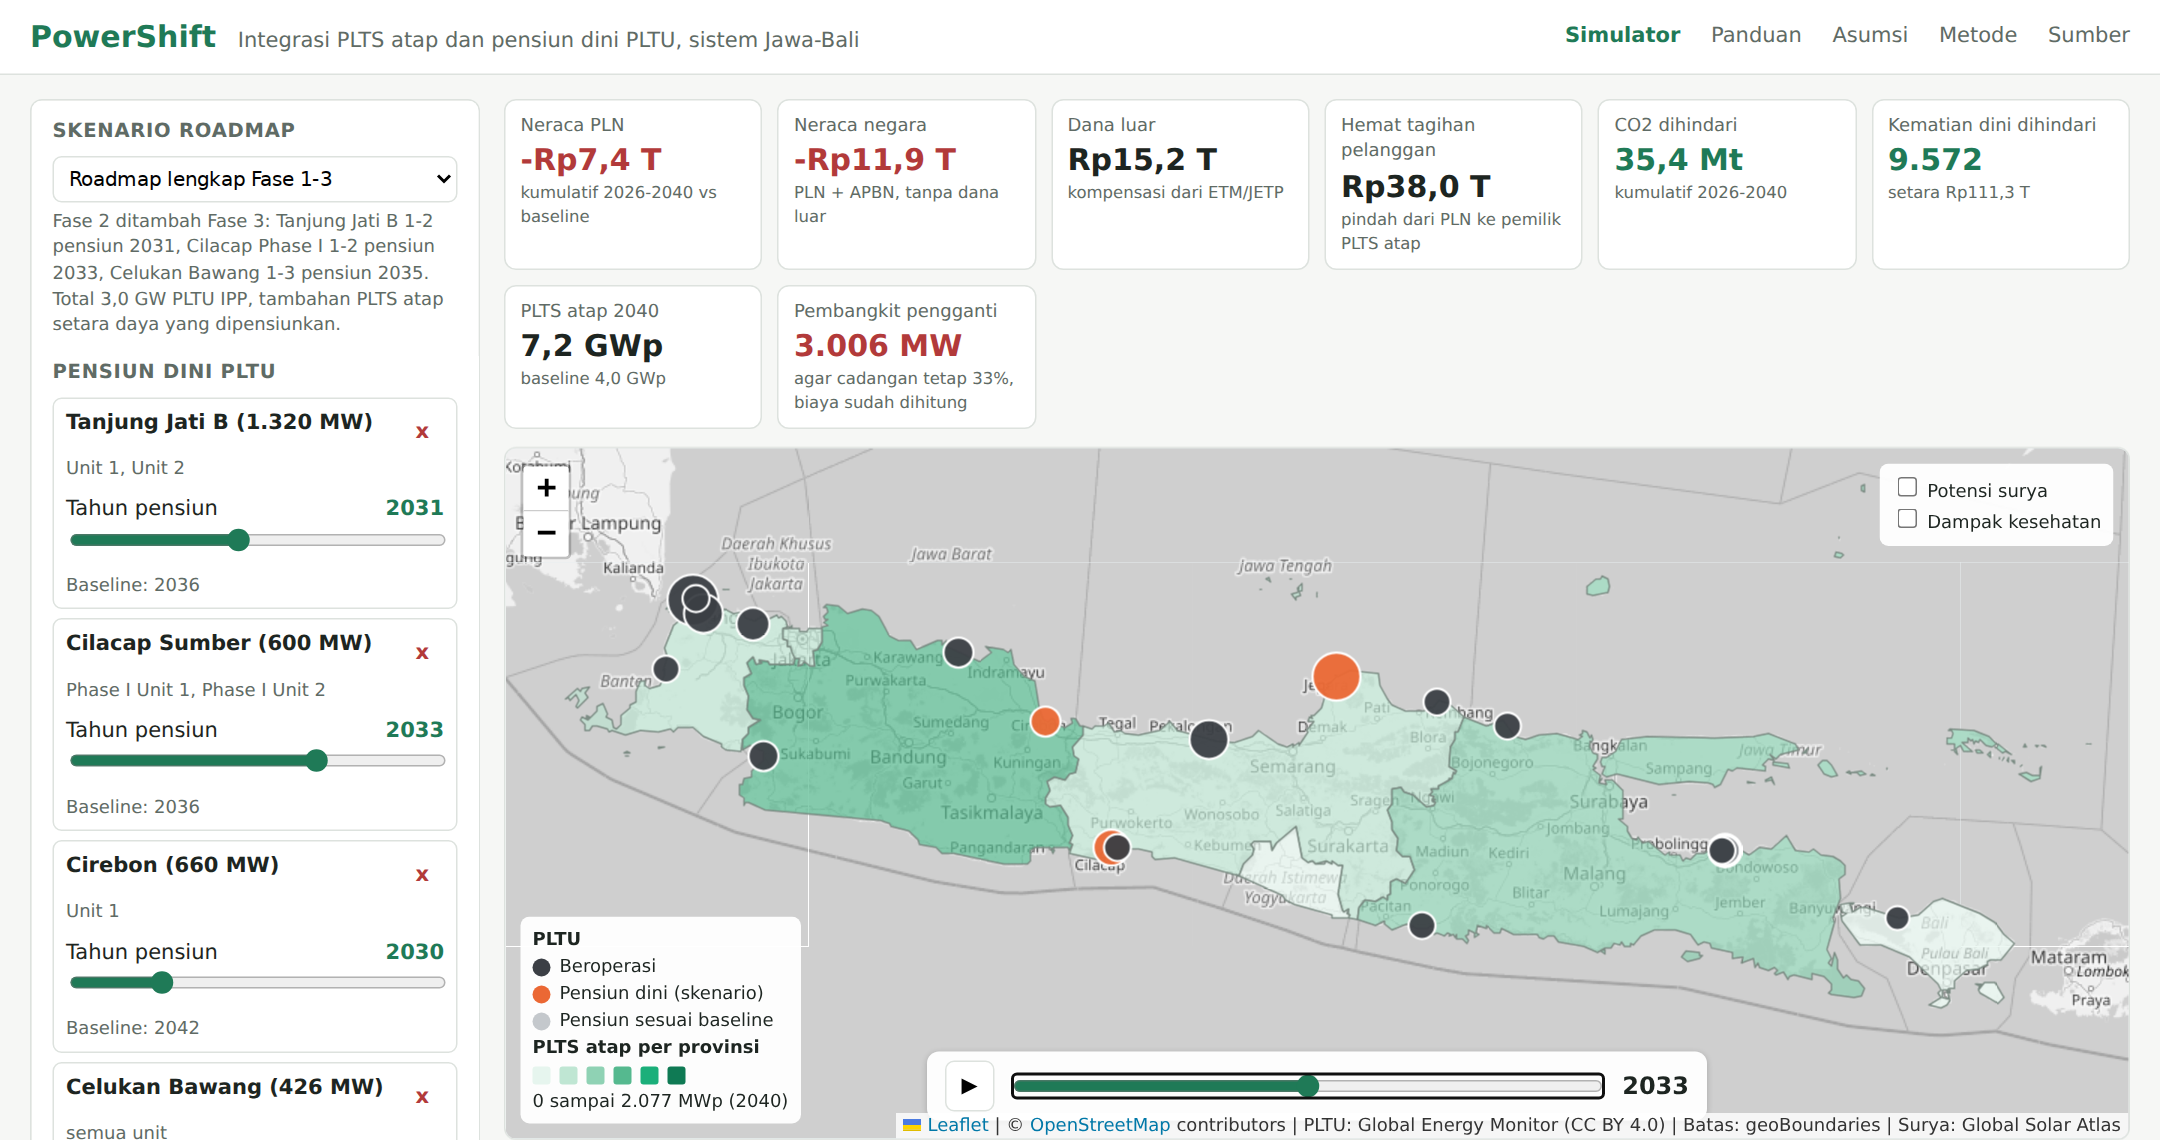
\includegraphics[width=\textwidth]{app_powershift}
\caption{Tampilan PowerShift pada skenario Roadmap Fase 1-3, tahun 2033}
\label{fig:app}
\sumber{\url{https://nazihnajmudin.github.io/Proyek-Periklim/}}
\end{figure}

\subsection{Kebaruan Program}

PLTS atap, pensiun dini, dan model neraca listrik masing-masing sudah dikenal. Kebaruan program ini terletak pada tiga hal. Pertama, kuota PLTS atap dikaitkan langsung dengan rencana pensiun dini sehingga PLTS atap dihitung sebagai pengganti. Kedua, urutan pensiun ditentukan oleh dampak terhadap neraca negara per GW, yang membedakan PLTU IPP dan PLTU milik PLN. Ketiga, seluruh penilaian dilakukan dengan alat terbuka yang memetakan biaya dan manfaat ke PLN, APBN, dana luar, pelanggan, dan kesehatan sekaligus.
